\documentclass[12pt,a4paper]{article}
\usepackage[french]{babel}
\usepackage[utf8x]{inputenc}
\usepackage[T1]{fontenc}
\usepackage{graphicx}
\usepackage[hidelinks]{hyperref}
\usepackage{fancyhdr}
\usepackage{pdflscape}
\usepackage{rotating}
\usepackage[margin=1in,headheight=15.0pt]{geometry}
\usepackage{listings}
\usepackage[usenames,dvipsnames,svgnames,table]{xcolor}
\usepackage{inconsolata}
\usepackage{enumitem}
\usepackage{float}
\usepackage{caption}
\usepackage{longtable}
\usepackage{array}
\usepackage{titlesec}


\title{SmartCity}
\author{Jérémy \textsc{Duchesne}\\Quentin \textsc{Lombat}\\Justin \textsc{Sirjacques}\\Noé \textsc{Picard}}
\date{\today}


%%%%%%%%%%%%%%%%%%%%%%%%%%%%%%%%%%%%%%%%%%%%%%%%%%%%%%%%%%%%%%%%%%%%%%%%%%%%%%%%%%%%%%%%%%%%%%%%%
%%%%%%%%%%%%%%%%%%%%%%%%%%%%%%%%%%%%%%% CUSTOMIZATION %%%%%%%%%%%%%%%%%%%%%%%%%%%%%%%%%%%%%%%%%%%
%%%%%%%%%%%%%%%%%%%%%%%%%%%%%%%%%%%%%%%%%%%%%%%%%%%%%%%%%%%%%%%%%%%%%%%%%%%%%%%%%%%%%%%%%%%%%%%%%
\makeatletter
\let\thetitle\@title
\let\theauthor\@author
\let\thedate\@date
\makeatother

% Custom header and footer
\pagestyle{fancy}
\fancyhf{}
\rhead{Groupe 8}
\chead{SmartCity}
\lhead{INFOM453}
\cfoot{Page \thepage}
\renewcommand{\headrulewidth}{0.4pt}
\renewcommand{\footrulewidth}{0.4pt}

\setlength{\parindent}{0pt}

% Customization for \begin{lstlisting} ('literate' option enables special character)
\lstset{
    basicstyle=\small\ttfamily,
    showstringspaces=false,
    commentstyle=\color{gray},
    keywordstyle=\color{blue},
    breaklines=true,
    numbers=left,
    numbersep=7pt,
    frame=single,
    numberstyle=\footnotesize,
    escapechar=\&,
    literate=
  {á}{{\'a}}1 {é}{{\'e}}1 {í}{{\'i}}1 {ó}{{\'o}}1 {ú}{{\'u}}1
  {Á}{{\'A}}1 {É}{{\'E}}1 {Í}{{\'I}}1 {Ó}{{\'O}}1 {Ú}{{\'U}}1
  {à}{{\`a}}1 {è}{{\`e}}1 {ì}{{\`i}}1 {ò}{{\`o}}1 {ù}{{\`u}}1
  {À}{{\`A}}1 {È}{{\'E}}1 {Ì}{{\`I}}1 {Ò}{{\`O}}1 {Ù}{{\`U}}1
  {ä}{{\"a}}1 {ë}{{\"e}}1 {ï}{{\"i}}1 {ö}{{\"o}}1 {ü}{{\"u}}1
  {Ä}{{\"A}}1 {Ë}{{\"E}}1 {Ï}{{\"I}}1 {Ö}{{\"O}}1 {Ü}{{\"U}}1
  {â}{{\^a}}1 {ê}{{\^e}}1 {î}{{\^i}}1 {ô}{{\^o}}1 {û}{{\^u}}1
  {Â}{{\^A}}1 {Ê}{{\^E}}1 {Î}{{\^I}}1 {Ô}{{\^O}}1 {Û}{{\^U}}1
  {œ}{{\oe}}1 {Œ}{{\OE}}1 {æ}{{\ae}}1 {Æ}{{\AE}}1 {ß}{{\ss}}1
  {ű}{{\H{u}}}1 {Ű}{{\H{U}}}1 {ő}{{\H{o}}}1 {Ő}{{\H{O}}}1
  {ç}{{\c c}}1 {Ç}{{\c C}}1 {ø}{{\o}}1 {å}{{\r a}}1 {Å}{{\r A}}1
  {€}{{\euro}}1 {£}{{\pounds}}1
}

\lstdefinelanguage{XML}
{
  morestring=[b]",
  morestring=[s]{>}{<},
  morecomment=[s]{<?}{?>},
  stringstyle=\color{black},
  identifierstyle=\color{blue},
  keywordstyle=\color{blue},
  morekeywords={xmlns,version,type,groupId,artifactId,scope}
}

\newcolumntype{x}[1]{>{\centering\let\newline\\\arraybackslash\hspace{0pt}}p{#1}}


\setcounter{secnumdepth}{4}

\titleformat{\paragraph}
{\normalfont\normalsize\bfseries}{\theparagraph}{1em}{}
\titlespacing*{\paragraph}
{0pt}{3.25ex plus 1ex minus .2ex}{1.5ex plus .2ex}


%%%%%%%%%%%%%%%%%%%%%%%%%%%%%%%%%%%%%%%%%%%%%%%%%%%%%%%%%%%%%%%%%%%%%%%%%%%%%%%%%%%%%%%%%%%%%%%%%
%%%%%%%%%%%%%%%%%%%%%%%%%%%%%%%%%%%%%%%%%% DOCUMENT %%%%%%%%%%%%%%%%%%%%%%%%%%%%%%%%%%%%%%%%%%%%%
%%%%%%%%%%%%%%%%%%%%%%%%%%%%%%%%%%%%%%%%%%%%%%%%%%%%%%%%%%%%%%%%%%%%%%%%%%%%%%%%%%%%%%%%%%%%%%%%%
\begin{document}

\begin{titlepage}
  \centering
  \vspace*{1 cm}
  
\includegraphics[scale = 0.3]{img/logo-unamur.png}\\[2.0 cm]
  \textsc{\large INFOM453 - Laboratoire en informatique ambiante et mobile}\\[0.5 cm]
  \textsc{\Large Rapport final}\\[0.5 cm]
  \rule{\linewidth}{0.2 mm} \\[0.4 cm]
  { \huge \bfseries \thetitle}\\
  \rule{\linewidth}{0.2 mm} \\[1.5 cm]

  \begin{minipage}[t]{0.4\textwidth}
    \begin{flushleft} \large
      \emph{Groupe 8:}\\
      \theauthor
    \end{flushleft}
  \end{minipage}~
  \begin{minipage}[t]{0.4\textwidth}
    \begin{flushright} \large
      \emph{Professeurs:} \\
      Bruno \textsc{Dumas}\\
      Pierre-Antoine \textsc{Rappe}
    \end{flushright}
  \end{minipage}\\[2 cm]
  \vfill
  {\large \thedate}\\[2 cm]

\end{titlepage}

\tableofcontents

\newpage
\section{Description du projet}
\subsection{3 tâches}
\begin{itemize}
    \item \textbf{Passer des zones routières en zones piétonnes et inversement :}\\
    Nous entendons par là la possibilité de rendre une partie de la ville (ou la ville dans son intégralité) piétonne. Cette mesure pourrait être de courte durée ou prolongée à long terme. Afin de réaliser cette première tâche, aucun capteur n’est réellement nécessaire, seuls des feux ainsi que des écrans d’affichage seraient nécessaires. Ces derniers permettraient de dévier les véhicules pour les faire contourner les zones devenues piétonnes et ainsi bloquer l’accès à celles-ci.
    \item \textbf{Prioritiser certains véhicules :}\\
    Cette deuxième tâche a pour but de privatiser certaines voies aux transports en commun afin que ceux-ci respectent le plus possible leurs horaires annoncés. Actuellement la plupart de ces voies sont réservées en permanence ce qui n’est pas une solution adéquate. En effet, les transports en commun circulent à des fréquences différentes en fonction des périodes de la journée et de l’année (ex. : vacances scolaires), il n’est donc pas nécessaire de constamment privatiser ces bandes. Ces dernières pourraient donc être partagées avec les usagers quotidiens afin de ne pas surcharger le réseau lorsque cela n’est pas nécessaire. Nous aurons désormais besoin de capteurs, notamment des capteurs de présence de véhicules afin de vérifier si le réseau est surchargé ou non. Des périphériques d’affichages seront également utiles afin de signaler aux usagers s’ils peuvent ou non circuler sur les bandes de bus.
    \item \textbf{Adapter la circulation en fonction d'événements ou de l’environnement :}\\
    Cette troisième et dernière tâche est la plus complexe. En effet, elle permet d’adapter le trafic en fonction de plusieurs critères tels que des événements (prévus : concerts, événements sportifs, etc. et non prévus : accidents de la route, etc.), la météo, le taux de pollution, etc. Plusieurs capteurs seront dès lors nécessaires, notamment des capteurs de température au sol, des capteurs de pollution, des capteurs de présence. De plus, afin d’être au courant des événements imprévus tels qu’un accident de la route, une interface utilisateur serait nécessaire (application mobile ou web). En plus de ces trois tâches principales, il va de soi que notre système gérera l’intégralité des feux de signalisation de la ville, ceci afin d’assurer un fonctionnement “classique” de ces feux (ex. : piétons souhaitant traverser).
\end{itemize}
\newpage
\subsection{Maquette}
\begin{figure}[H]
    \begin{center}
        \frame{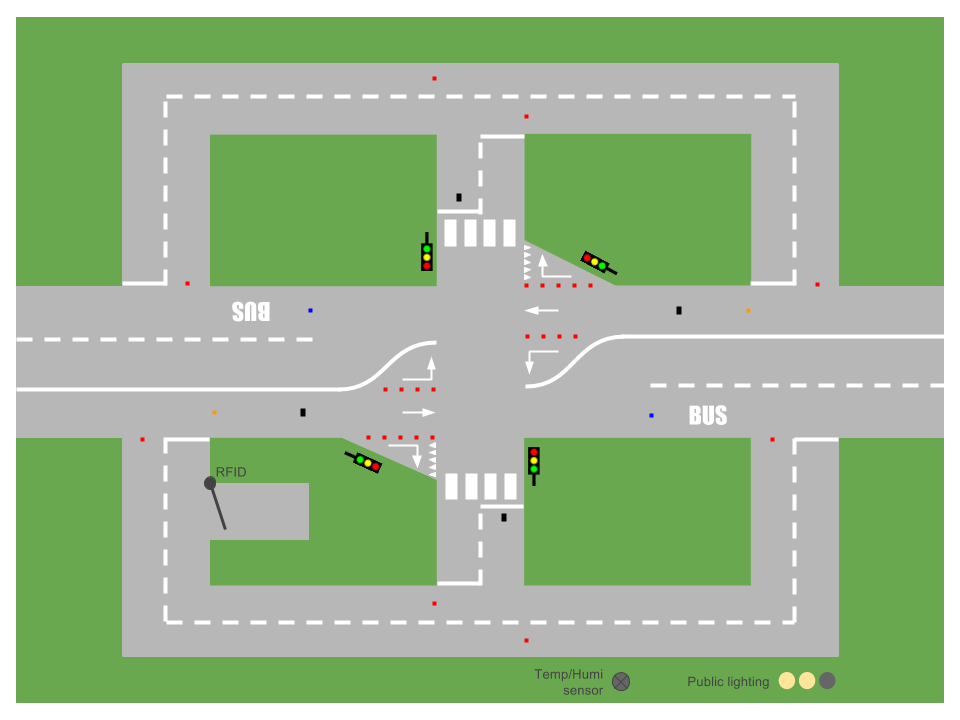
\includegraphics[width=\linewidth, height=\textheight,keepaspectratio]{img/maquette}}

        \caption{Croquis de la maquette}\label{croquis-maquette}
    \end{center}
\end{figure}
\vspace{-0.7cm}
Afin de pouvoir utiliser les senseurs de manière optimale, nous avons imaginé la maquette telle que ci-dessus (illustration \ref{croquis-maquette}). Les LEDs rouges représentent des interdictions. Lorsqu’elles sont allumées, les automobilistes ne peuvent pas aller dans ces rues. Les deux LEDs bleues sont pour les bandes de bus. Allumées, elles indiquent que la bande est réservée aux bus, et donc que les autres usagers doivent tous se rabattre sur la seconde bande. Le RFID est utilisé comme entrée d’un parking (ici, dans la partie inférieure gauche de la maquette).

\section{Projet squelette}
Au début du projet, il nous a été demandé de respecter un certain nombre de critères bien particuliers. Voici comment nous les avons intégrés au projet.\\

Tout d’abord, en ce qui concerne les Phidgets, nous devions utiliser au moins une Phidget board. Cela était indispensable, notre projet ne pouvant pas se passer de l’Interface Kit. Nous avions également comme consigne de récupérer l’information provenant d’au moins deux capteurs. Le système actuel récupère et utilise les informations de deux capteurs de distance IR (sur l’axe principal, pour détecter les voitures), deux capteurs de luminosité (sur l’axe auxiliaire, pour détecter les voitures. Nous n’avions pas assez de capteurs de distance IR pour les deux axes), d’un capteur de luminosité, d’un capteur d’humidité, ainsi que d’un lecteur de tag RFID. Ce dernier, combiné avec le moteur, est utilisé comme ouverture de parking. La barrière s’ouvre si l’utilisateur a payé son droit d’entrée au parking.\\

Ensuite, il était demandé de créer une couche Scala qui traiterait les données récupérées par les capteurs. Nous avons décidé d’écrire entièrement le code en Scala. En effet, tout notre système fonctionnant sous la forme de Threads interdépendants qui doivent communiquer entre eux, il nous a semblé évident d’utiliser les Acteurs de la librairie Akka pour gérer ces Threads. Il sera expliqué plus précisément comment fonctionne nos acteurs plus loin dans ce rapport (cf. \ref{systeme-acteurs}). Un autre point important était qu’il fallait agréger l’information de deux capteurs et en déduire une information particulière. Nous avons donc récupéré la température ainsi que l’humidité, et pouvons en déduire l’état de la route afin d’ajuster la vitesse. Bien que les limites soient très facilement modifiables, pour le moment la vitesse de base est 50 km/h dans toute la ville. Lorsque la température descend en dessous des 3 degrés, et que l’humidité dépasse les 70\%, la vitesse passe à 30 km/h, parce que le risque de verglas est important. Nous proposons également un web service API, qui permet de récupérer les informations de notre base de données, mais également d’effectuer des modifications, telles qu’ouvrir une zone particulière de la ville, ou ajouter une nouvelle zone. Il en va de même pour les horaires de bus, qui sont modifiables et supprimables depuis l’API.\\


\newpage
\section{Architecture matérielle}
Avant toute explication, voici le schéma muni d’annotations afin d’identifier plus facilement chaque élément matériel.\\

\begin{figure}[H]
    \begin{center}
        \frame{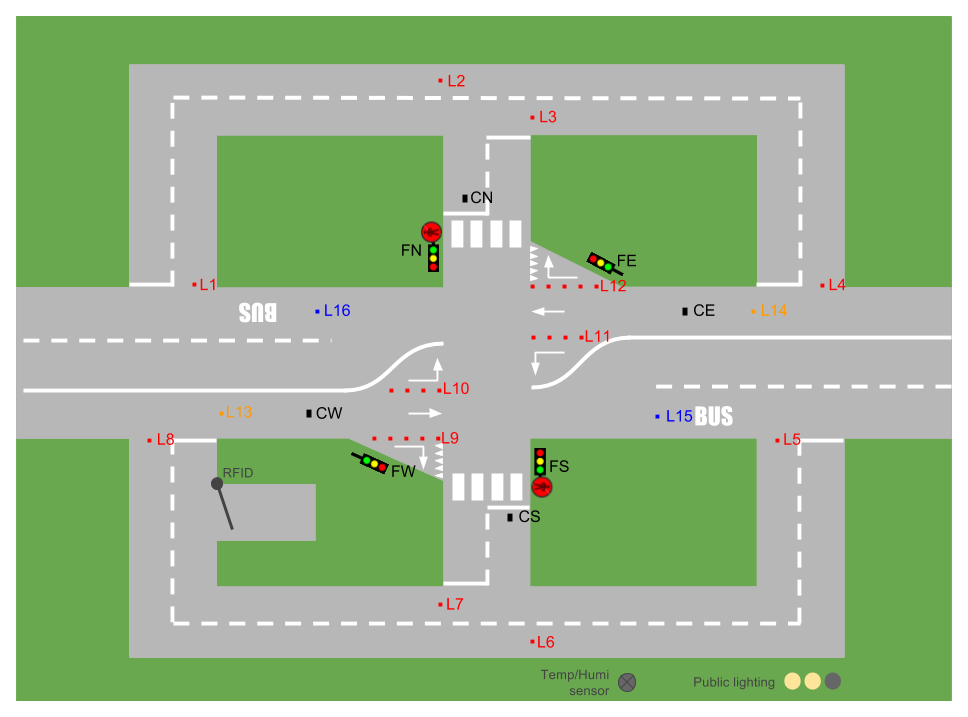
\includegraphics[width=\linewidth, height=\textheight,keepaspectratio]{img/maquette-materiel}}

        \caption{Croquis de la maquette}
    \end{center}
\end{figure}

La partie hardware sera divisée en deux parties principales. Dans un premier temps, l’arduino et l’ensemble des capteurs, des leds et des affichages lui étant connectés seront abordées. Deuxièmement, l’ensemble des interfaces Phidgets vous seront détaillées, évidemment les précisions les plus précises seront apportées à l’InterfaceKit 8/8/8 qui a recueilli une multitude de capteurs et de leds.\\

\subsection{Arduino}
\subsubsection{Élément connectés}
\subsubsection{Détails techniques}

\subsection{Phidgets}
\subsubsection{InterfaceKit 8/8/8}
\subsubsection{Advanced Servo 1-Motor}
\subsubsection{RFID Read-Write}




\newpage
\section{Architecture logicielle}
Le diagramme suivant représente les élément logiciels les plus importants de notre architecture. Ces différents composants sont décrits en détail dans les sections suivantes.
\begin{figure}[H]
    \begin{center}
        \frame{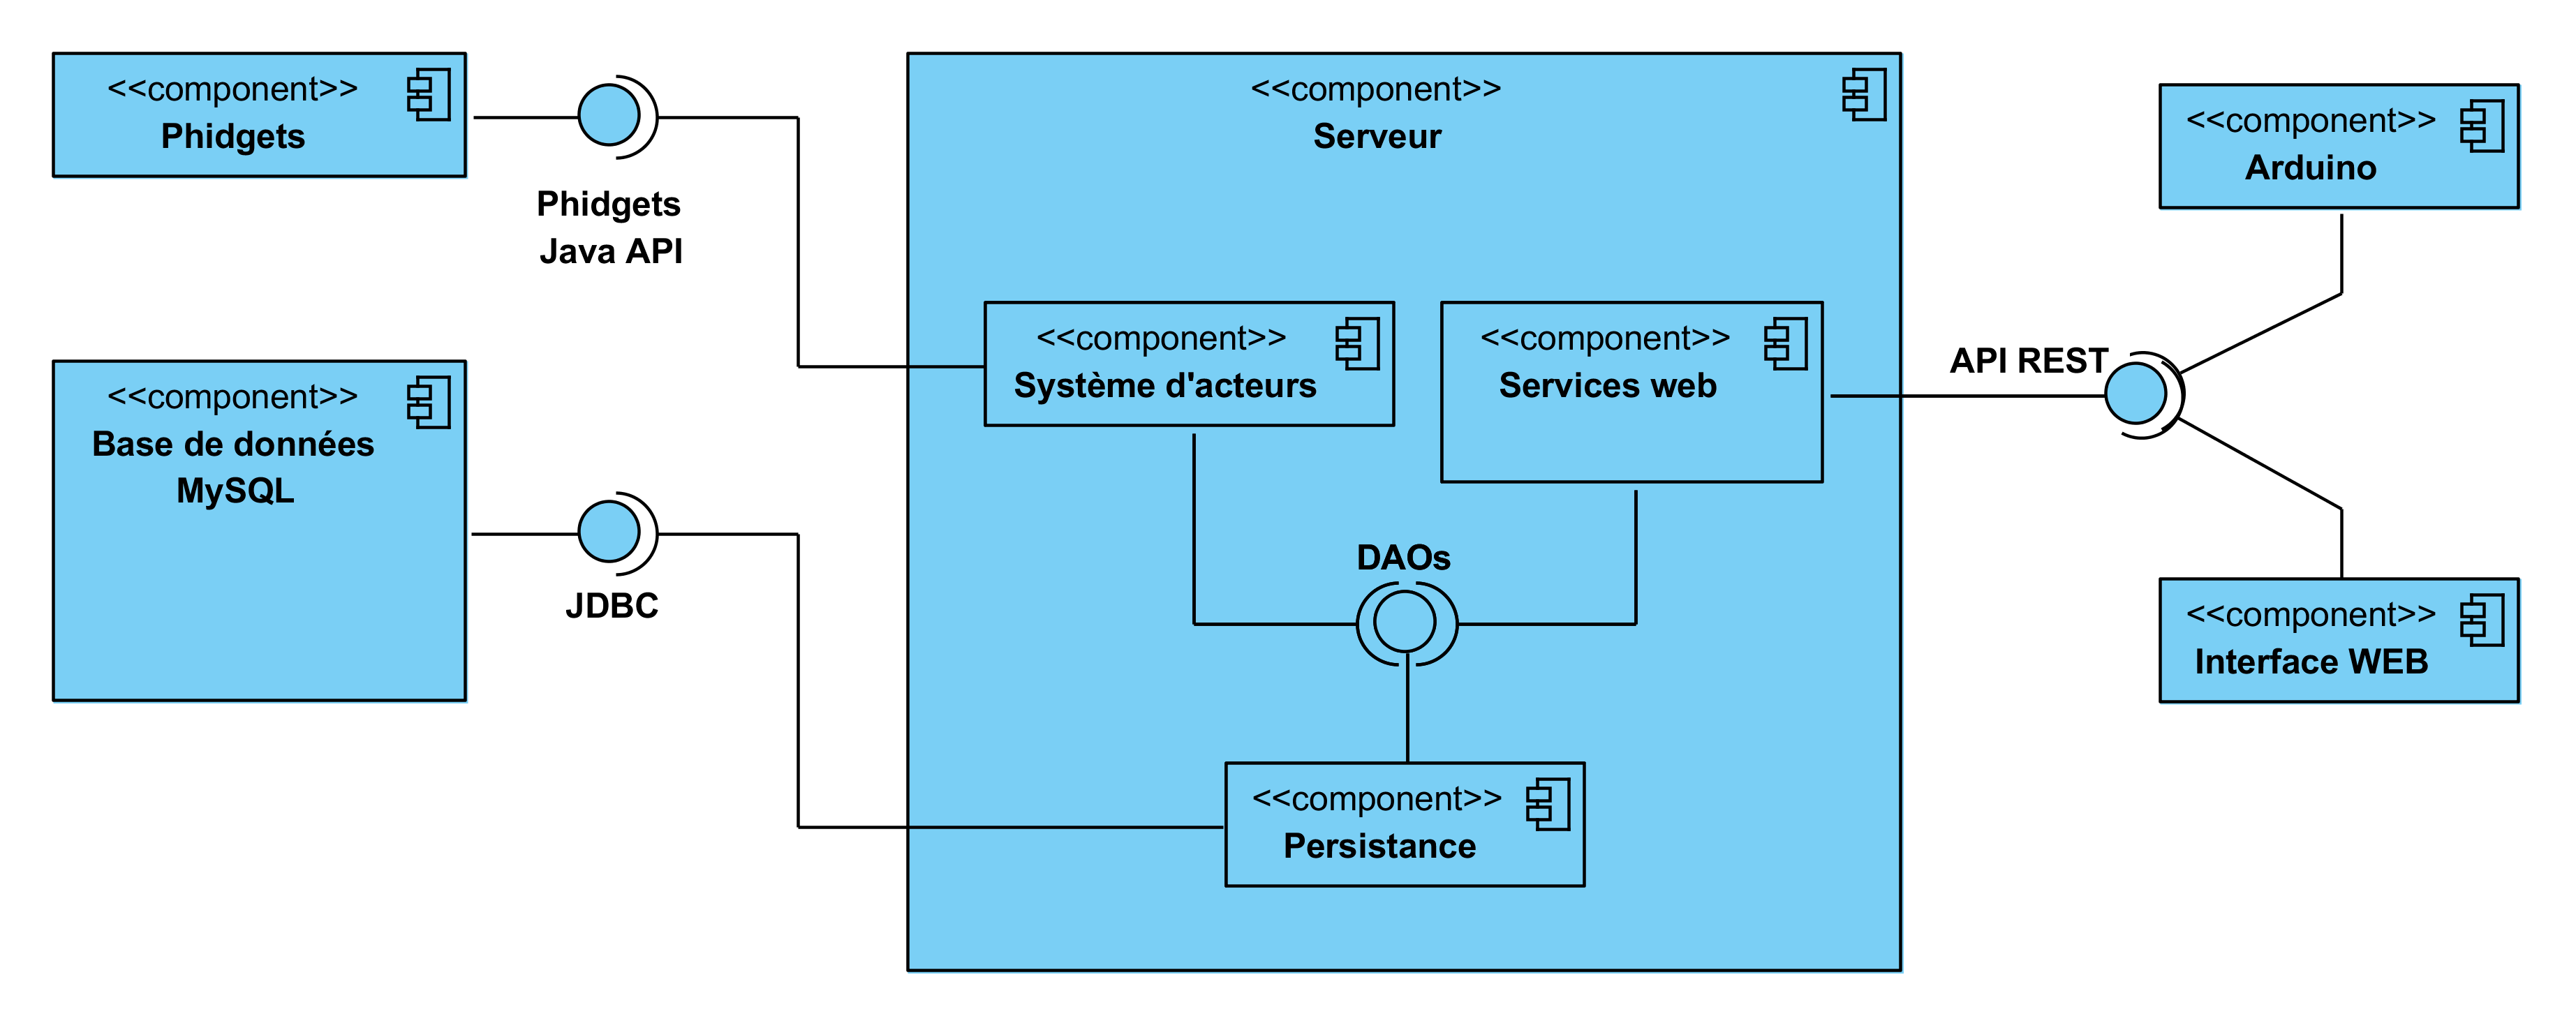
\includegraphics[width=\linewidth, height=\textheight,keepaspectratio]{img/diagramme-composants-archi-logi}}

        \caption{Diagramme de composants de l'architecture logicielle}
    \end{center}
\end{figure}
\subsection{Serveur}
Notre architecture logicielle côté serveur est basée sur une pile applicative reposant entièrement sur le langage Scala. Nous nous attarderons ici à décrire les 3 composants regroupés dans le serveur.\\

Néanmoins, quelques remarques préliminaires sont nécessaires :
\begin{itemize}
\item Pour faciliter le développement et surtout la gestion des dépendances, nous avons utilisé Maven. Lors de la phase de développement, le conteneur de servlets Jetty était utilisé. En phase de déploiement, nous avons choisi d’utiliser Tomcat 8 sur le Raspberry Pi (le WAR pouvant être facilement généré grâce à la commande : mvn:package).
\item Comme la librairie Java pour le Phidgets n’est pas disponible au travers d’un dépôt maven, il est nécessaire de l’importer localement sur la machine. Les instructions pour y parvenir sont disponibles en annexe.
\item Pour déployer le projet sur une machine de développement, il suffit d’exécuter la commande maven : mvn:jetty. En ce qui concerne le déploiement sur le Raspberry Pi, il est uniquement nécessaire de transférer le fichier WAR (préalablement généré) dans le dossier ‘webapps’ de Tomcat (l’auto-déploiement étant supposé activé).\\
\end{itemize}

Afin d’être complet, voici le diagramme de classes du composant \emph{Serveur} :
\begin{figure}[H]
    \begin{center}
        \frame{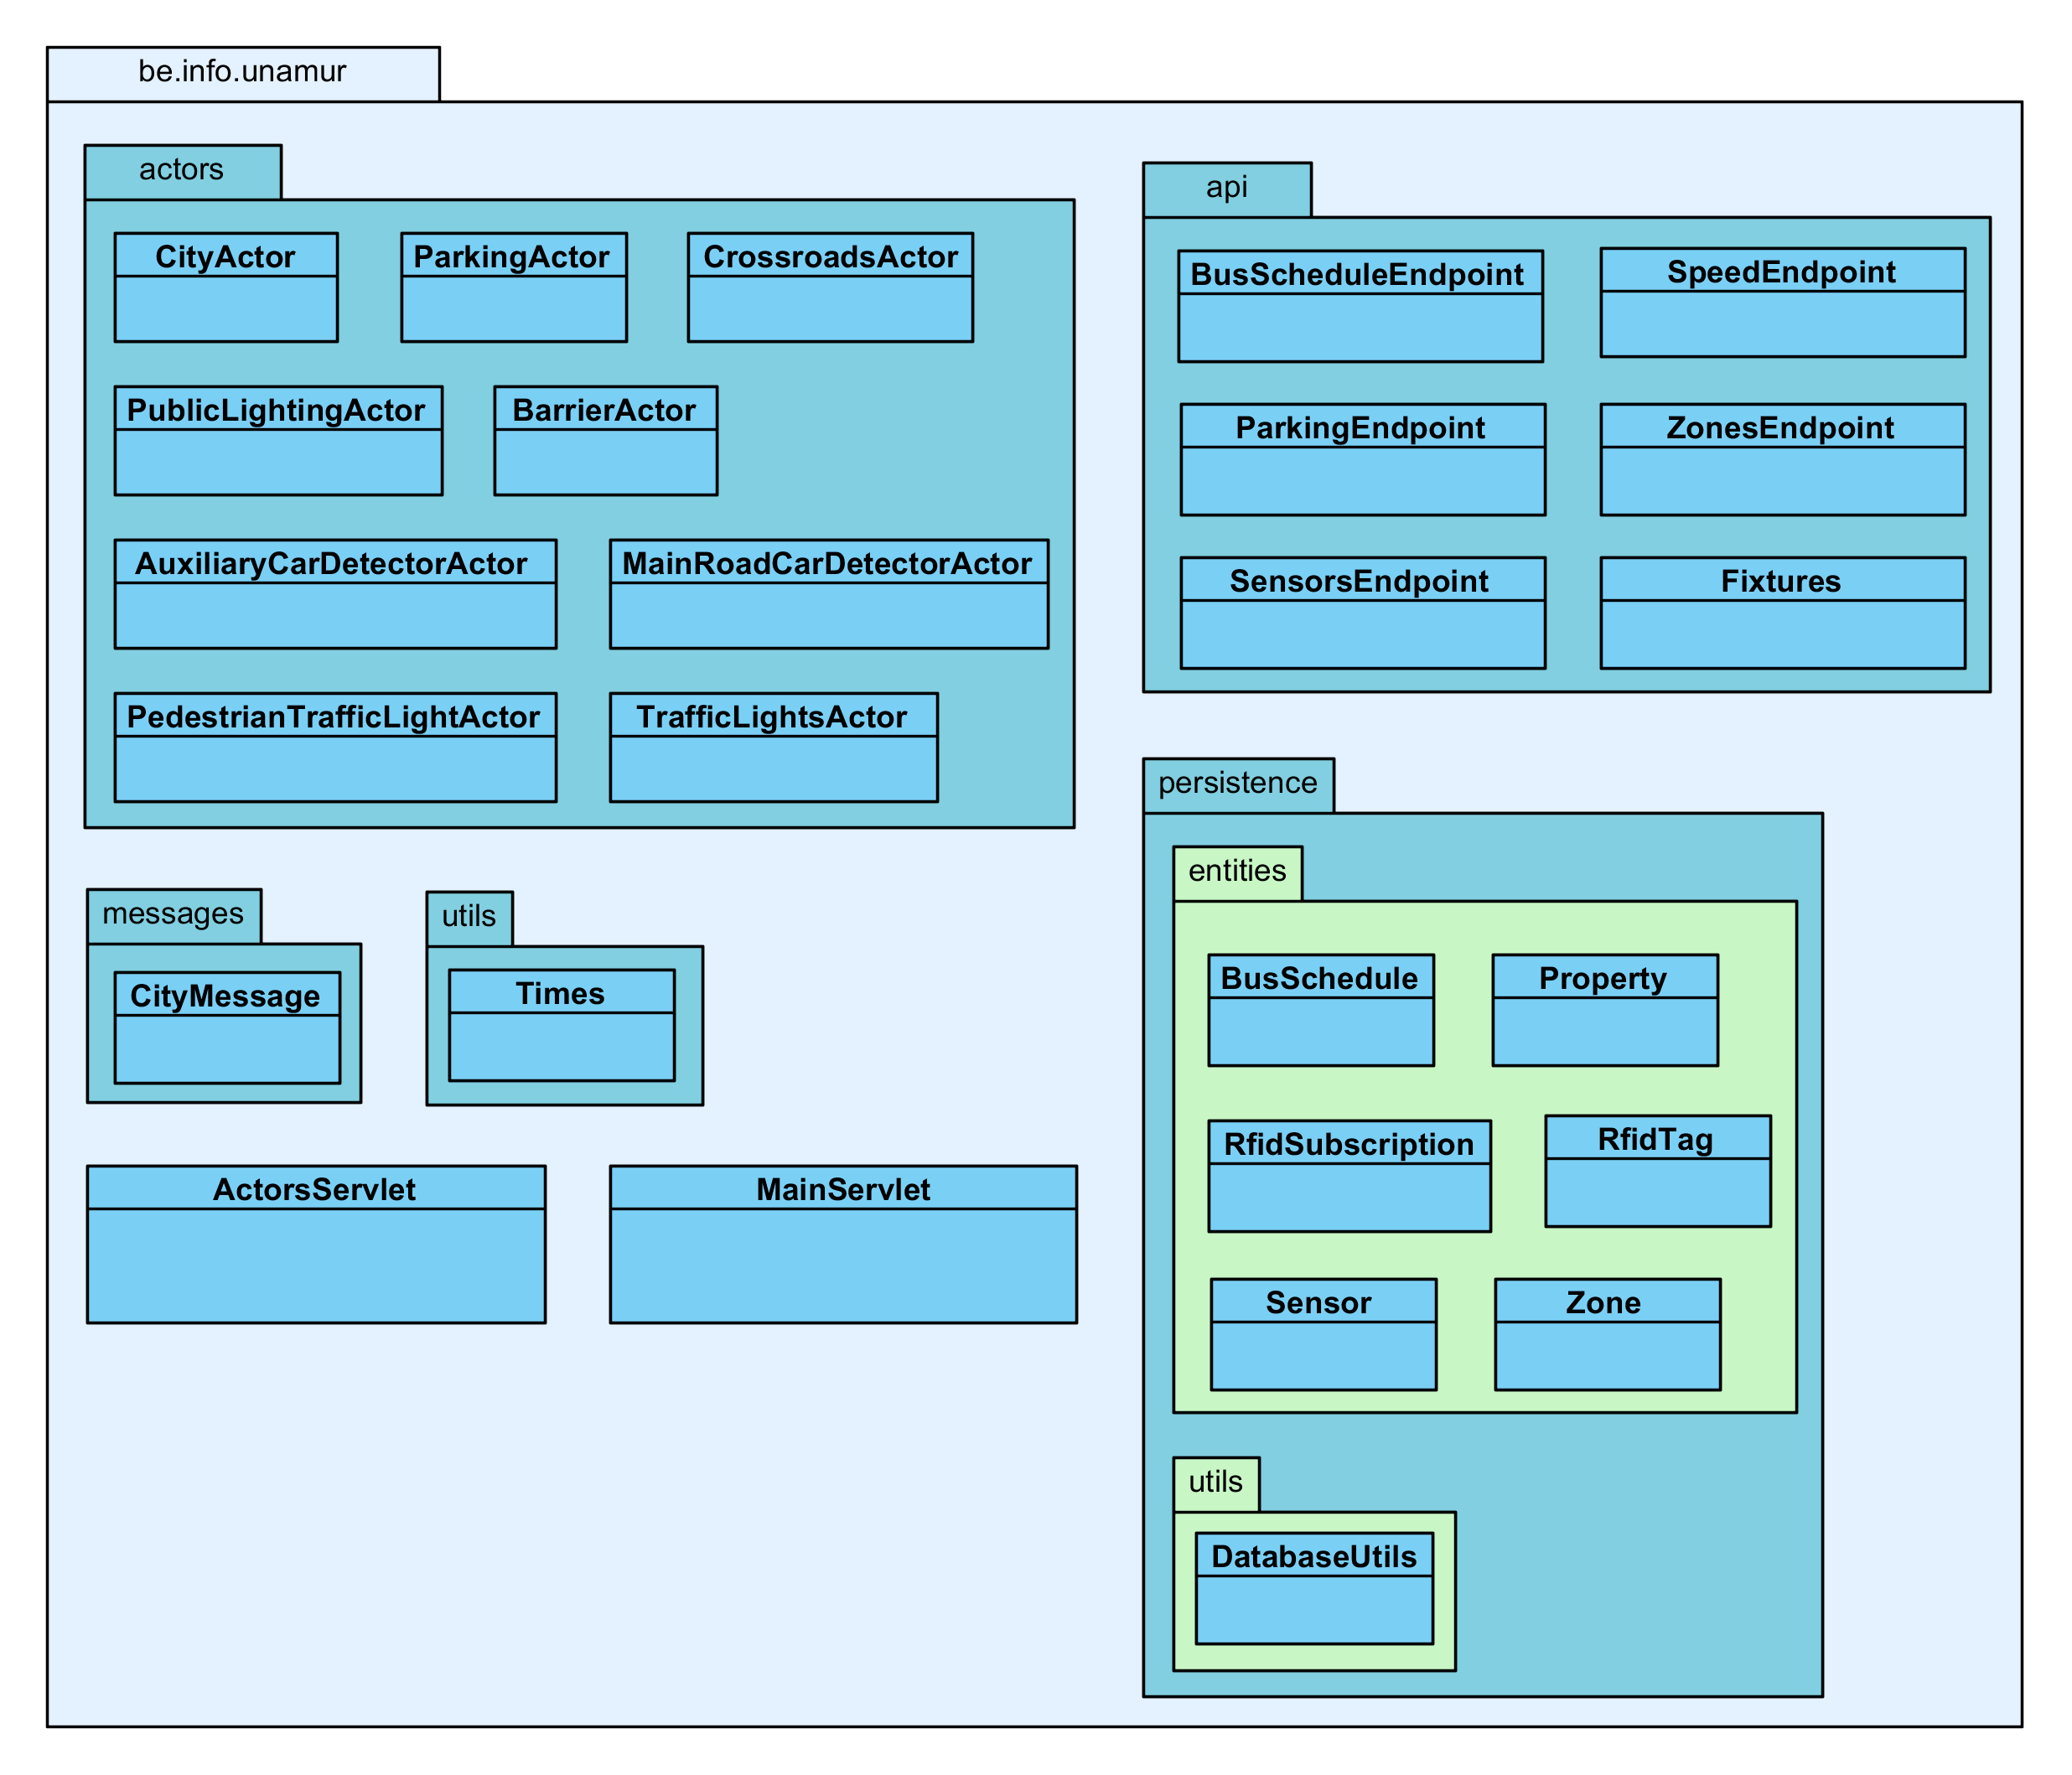
\includegraphics[width=\linewidth, height=\textheight,keepaspectratio]{img/diagramme-class-archi-logi}}

        \caption{Diagramme de class de l'architecture logicielle}
    \end{center}
\end{figure}

Intéressons-nous maintenant aux 3 composants principaux : le système d’acteurs, les services web et la « persistance » (c.-à-d. l’interaction avec la base de données).


\subsubsection{Système d'acteurs}\label{systeme-acteurs}
Pour contrôler le matériel (c.-à-d. les phidgets décrits ci-avant qui sont connectés au Raspberry Pi), nous basons la notion d’Acteurs proposée par la librairie Akka. Ainsi, chaque concept physique (la ville, le carrefour, les feux de signalisations, etc.) de notre maquette est représenté par un acteur. Cela nous a permis de faciliter grandement le code, de le rendre plus modulable et facile à faire évoluer.
Ce système d’Acteurs s’organise sous la forme d’un arbre qui peut être représenté de la façon suivante :
\begin{figure}[H]
    \begin{center}
        \frame{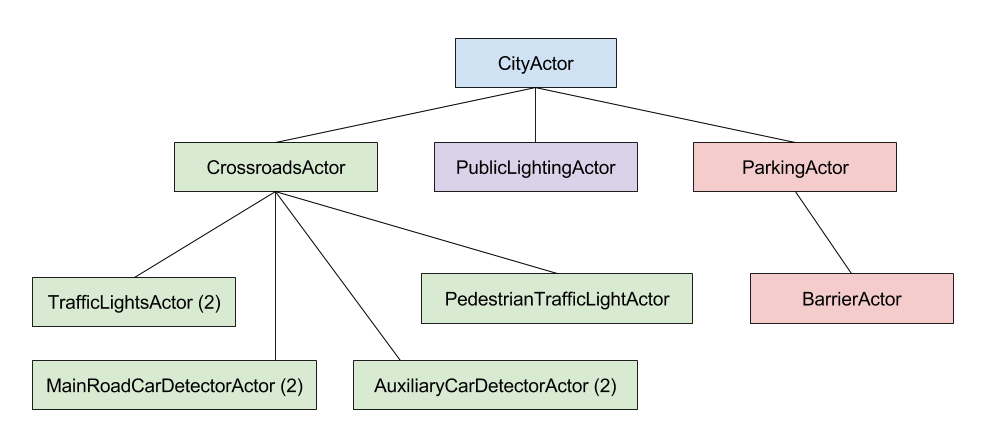
\includegraphics[width=\linewidth, height=\textheight,keepaspectratio]{img/systeme-acteurs-archi-logi}}

        \caption{Structure du système d'acteurs}
    \end{center}
\end{figure}
On remarque donc que la ville (\emph{CityActor}) est l’acteur principal ou aussi appelé le « maître », c’est lui qui est à la racine de notre système. Les sous-acteurs engendrés par celui-ci sont des composants plus petits à l’intérieur de la ville, c’est-à-dire le carrefour (\emph{CrossroadsActor}), le parking (\emph{ParkingActor}) et l’éclairage public (\emph{PublicLightingActor}).\\

Tout d’abord, il faut noter qu’il est possible de démarrer et d’arrêter tout le système d’acteurs. Ceci est réalisé en envoyant le message \emph{Initialize} à l’acteur principal qui va ensuite le propager dans tout l’arbre d’acteurs. De la même façon, s'ils ont été démarrés auparavant, il est possible de les stopper en envoyant le message \emph{Stop} à l’acteur principal qui le propagera de la même façon que pour le message de démarrage. Le fait d’initialiser des acteurs va ouvrir les connexions aux phidgets nécessaires, mais aussi ajouter les listeners et mettre en place une situation initiale (les feux de la voie principale au vert et ceux des auxiliaires au rouge). Stopper les acteurs fera l’effet inverse.\\

Ensuite, l’acteur du carrefour pilote tous les composants nécessaires au bon fonctionnement du celui-ci :
\begin{itemize}
\item Les détecteurs de voitures sur la voie principale (\emph{MainRoadCarDetectorActor}). Comme expliqué dans la partie concernant le matériel, ces détecteurs sont au nombre de deux, un pour la voie principale côté Ouest et un pour la voie principale côté Est. Il y aura donc bien deux instanciations de l’acteur \emph{MainRoadCarDetectorActor}.
\item Les détecteurs de voitures sur la voie auxiliaire (\emph{AuxiliaryCarDetectorActor}). Similairement aux détecteurs de voitures, il existe deux capteurs, un pour le Nord et un pour le Sud, et donc deux instanciations de l’acteur \emph{AuxiliaryCarDetectorActor}.
\item Les feux de signalisations pour les voitures (un acteur \emph{TrafficLightsActor} par feu). Sur notre maquette, il existe 4 feux mais ceux des voies auxiliaires (Nord et Sud) et ceux des voies secondaires (Ouest et Est) fonctionnent respectivement en parallèle, uniquement deux instanciations de l’acteur \emph{TrafficLightsActor} sont dès lors nécessaires.
\item Les feux de signalisations pour les piétons (un acteur \emph{PedestrianTrafficLightActor} par feu). Uniquement les voies auxiliaires sont équipées de feux pour piétons fonctionnant en parallèle, il y aura donc une seule instanciation de l’acteur \emph{PedestrianTrafficLightActor}.
\end{itemize}

Le contrôle du carrefour part principalement de l’acteur qui gère celui-ci, en envoyant des messages aux sous-acteurs pour déléguer le travail (allumer et éteindre des feux, vérifier l’état des détecteurs de présences, etc.).\\

L’acteur pour le parking s’occupe principalement du lecteur RFID et aussi de contrôler la barrière en envoyant des messages à l’acteur correspondant à celle-ci (\emph{BarrierActor}). Ainsi, grâce à un listener sur le lecteur RFID, lorsqu’un tag est lu, si celui-ci est enregistré dans la base de données (voir ci 2.2.1.3), l’acteur envoie le message d’ouverture de la barrière du parking à l’acteur concerné. Quand le tag est perdu, il envoie le message de fermeture.\\

L’acteur pour l’éclairage public allume et éteint lorsqu’il est nécessaire les LEDs représentant ce même éclairage sur la maquette. Pour ce faire, un listener écoute les valeurs du capteur de luminosité et allume ou éteint certaines LEDs. Par exemple, si la valeur renvoyée par le capteur est élevée, les 3 LEDs seront allumées et inversement dans l’autre cas mais aussi avec des valeurs intermédiaires pour allumer 1 ou 2 LEDs.\\

Enfin, tous les messages échangés entre les acteurs sont définis dans la “case class” \emph{CityMessage}.


\subsubsection{Services web (API REST)}
L’API REST que nous avons mise en place est implémentée en se basant intégralement sur les outils proposés par Scalatra. Ainsi, il est facile de rajouter de nouveau point d’accès ou d’en supprimer. De plus la documentation de celle-ci est disponible sous format JSON et peut être visualisée en utilisant l’outil Swagger UI (c’est aussi pourquoi nous ne nous attarderons pas à documenter ici toute l’API).\\

Les points d’accès principaux sont les suivants :
\begin{center}
{\renewcommand{\arraystretch}{1.5}
\begin{longtable}{| p{.35\textwidth} | p{.59\textwidth} |}
    \hline
    \textbf{Nom} & \textbf{Description}\\
    \hline
    \emph{BusScheduleEndpoint} & Permet de récupérer et de modifier les informations des horaires de bus au sein de la ville.\\
    \hline
    \emph{ParkingEndpoint} & Permet de récupérer certaines informations concernant le parking (comme l’historique d’entrées/sorties ou le nombre de places disponibles).\\
    \hline
    \emph{SensorsEndpoint} & Donne accès aux informations concernant tous les capteurs implantés dans la ville : luminosité, présence, température, humidité, ...\\
    \hline
    \emph{SpeedEndpoint} & Sert principalement à récupérer la vitesse courante au sein de la ville.\\
    \hline
    \emph{ZonesEndpoint} & Permet de fermer et d’ouvrir certaines zones mais aussi de connaître lesquelles sont fermées. Un historique des fermetures et des ouvertures est également disponible.\\
    \hline
    \caption{Points d'accès de l'API REST}
\end{longtable}}
\end{center}
\vspace{-1cm}

\subsubsection{Persistence}
Pour communiquer avec notre base de données MySQL, nous nous somme appuyés sur la librairie ScalikeJDBC. Dans le package nommé \emph{entities}, se trouvent donc toutes les DAO nécessaires (chaque DAO correspondant à une table dans la base de données) :
\begin{center}
{\renewcommand{\arraystretch}{1.5}
\begin{longtable}{| p{.69\textwidth} | x{.25\textwidth} |}
    \hline
    \textbf{Nom} & \textbf{Schéma}\\
    \hline
    \emph{BusSchedule} (correspond à la table 'bus\_schedule') &
    \begin{minipage}{\linewidth}
        \centering
        \vspace{12pt}
        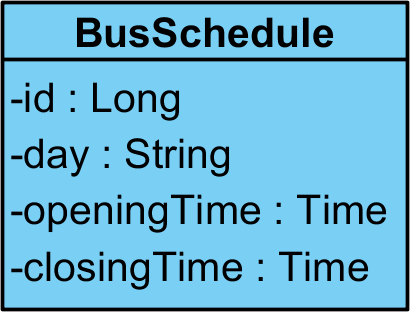
\includegraphics[scale=0.8]{img/bus-schedule}\par
        \vspace{12pt}
    \end{minipage}\\
    \hline
    \emph{Property} (correspond à la table 'property') &
    \begin{minipage}{\linewidth}
        \centering
        \vspace{12pt}
        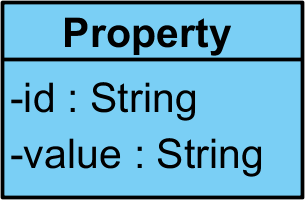
\includegraphics[scale=0.8]{img/property}\par
        \vspace{12pt}
    \end{minipage}\\
    \hline
    \emph{RfidSubscription} (correspond à la table 'rfid\_subscription') &
    \begin{minipage}{\linewidth}
        \centering
        \vspace{12pt}
        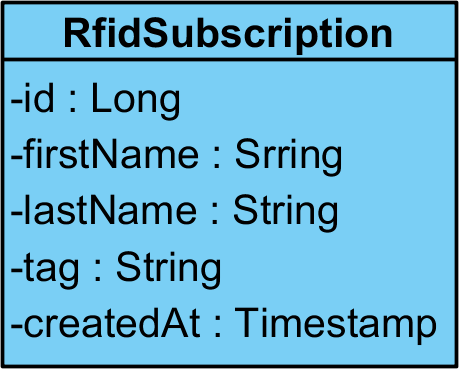
\includegraphics[scale=0.8]{img/rfid-sub}\par
        \vspace{12pt}
    \end{minipage}\\
    \hline
    \emph{RfidTag} (correspond à la table 'rfid\_tag') &
    \begin{minipage}{\linewidth}
        \centering
        \vspace{12pt}
        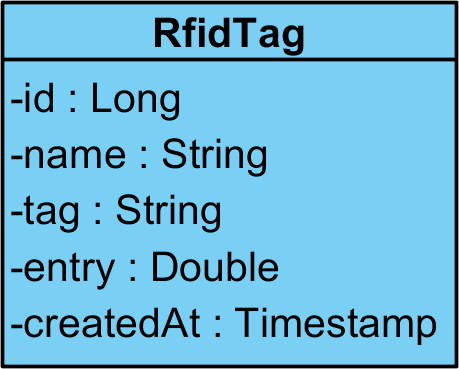
\includegraphics[scale=0.8]{img/rfid-tag}\par
        \vspace{12pt}
    \end{minipage}\\
    \hline
    \emph{Sensor} (correspond à la table 'sensor') &
    \begin{minipage}{\linewidth}
        \centering
        \vspace{12pt}
        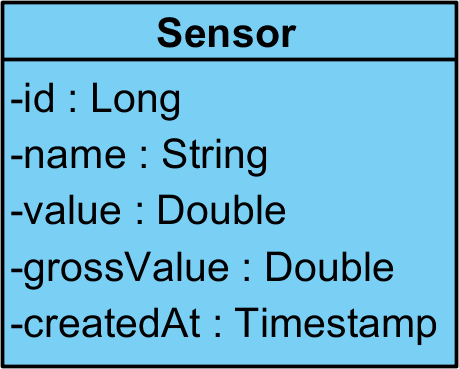
\includegraphics[scale=0.8]{img/sensor}\par
        \vspace{12pt}
    \end{minipage}\\
    \hline
    \emph{Zone} (correspond à la table 'zone') &
    \begin{minipage}{\linewidth}
        \centering
        \vspace{12pt}
        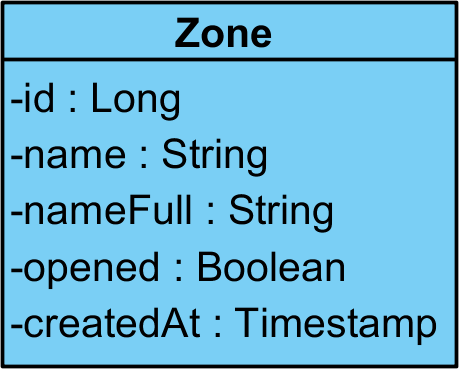
\includegraphics[scale=0.8]{img/zone}\par
        \vspace{12pt}
    \end{minipage}\\
    \hline
    \caption{Entités de la base de données}
\end{longtable}}
\end{center}
\vspace*{-0.7cm}
Les méthodes CRUD (et quelques autres qui nous sont utiles) se trouvent dans les objets "companions" correspondants à chaque DAO.
\subsection{Arduino}
\subsubsection{But de l'Arduino}
\subsubsection{Gestion des zones}
\subsubsection{Recevoir et envoyer des informations}
\subsubsection{Méthodes et fonctions}



\newpage
\section{Application à la réalité}
Translater notre système, actuellement dans une situation de carrefour parfait, dans une situation de carrefour mal fait, est possible. Sous contrainte que nous disposions d’un plus grand nombre de senseurs, il serait envisageable de rendre un carrefour illogique plus optimisé. Prenons un exemple concret :

\begin{figure}[H]
    \begin{center}
        \frame{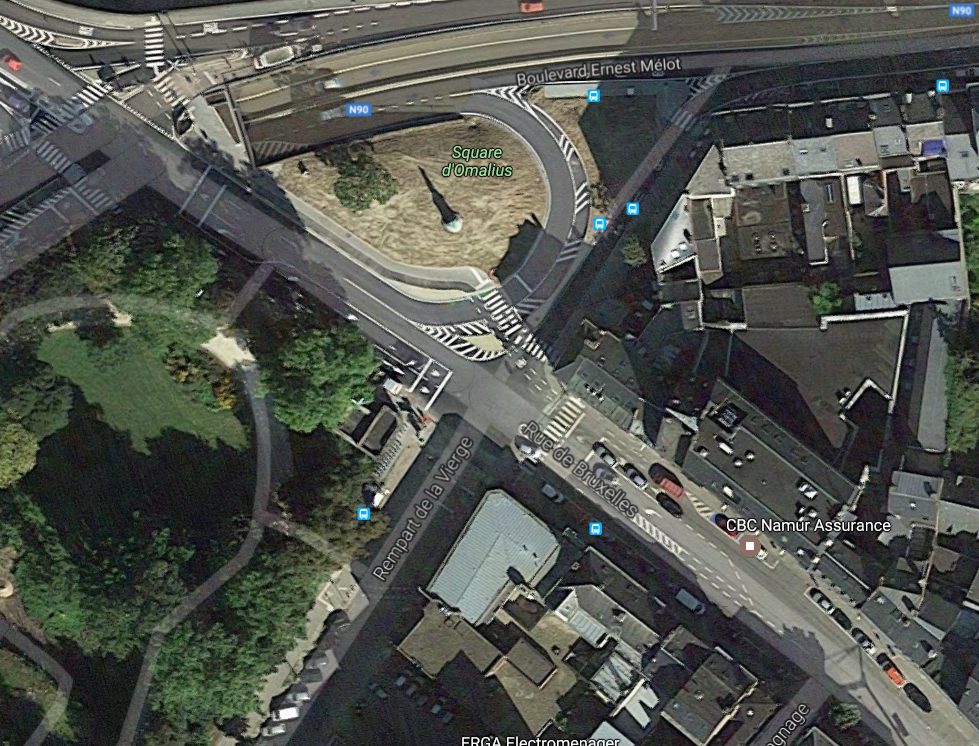
\includegraphics[width=\linewidth, height=\textheight,keepaspectratio]{img/application-realite}}

        \caption{Carrefour non loin des facultés de l'UNamur}
    \end{center}
\end{figure}

Comme nous pouvons le constater, il y a des voies provenant d’un peu partout. La N90 permet deux entrées dans le carrefour : soit le long du parc Louise-Marie, soit par le Square d’Omalius après être passé sous le carrefour. Des véhicules proviennent également de la rue de Bruxelles, de l’Avenue des Combattants ainsi que du Rempart de la Vierge. A noter que les véhicules provenant de la N90 par le parc Louise-Marie peuvent tourner dans toutes les directions, alors que ceux provenant du Square d’Omalius sont obligés de se diriger vers l’Avenue des Combattants. Les véhicules venant du nord par la N90 et se dirigeant vers l’Avenue des Combattants, ainsi que ceux provenant de cette dernière et allant vers le sud par la N90 ne sont pas repris dans le carrefour, puisqu’ils doivent respecter le principe du “Cédez le passage”.

Notre solution repose sur le fait qu’une voie est prioritaire par rapport aux autres afin d’optimiser le passage sur la principale. Dans le cas présent, le gros de la circulation provient des deux entrées de la N90 et se dirige en grosse partie vers l’Avenue des Combattants. Il arrive également souvent qu’il n’y ai pas de voitures provenant de la Rue de Bruxelles et du Rempart de la Vierge, malgré que leur feu soit vert. Il serait dès lors possible d’avantager les deux entrées de la N90 par rapport aux autres voies. Tout comme sur notre maquette actuelle, des capteurs de présence nous permettraient d’évaluer la présence sur les autres axes, et de ne mettre au rouge les entrées de la N90 que lorsque des voitures se présentent sur ces axes.

De plus, de la même manière que nous pouvons conseiller aux usagers d’emprunter un chemin différent sur la maquette, nous pourrions ici détecter un embouteillage sur l’une des entrées de la N90 sur le carrefour, et conseiller aux automobilistes d’utiliser l’autre.

Au niveau du code, la translation vers ce carrefour serait très facile. Comme nous fonctionnons avec les acteurs, il suffirait de déclarer autant d’acteurs “Feu rouge” dans l’acteur “Carrefour” qu’il y a réellement de feux, et adapter les temps d’attente minimum de chaque axe.


\newpage
\section{Annexes}
\subsection{Importer la librairie Java Phidgets dans Maven}
\begin{itemize}
\item Télécharger la documentation de la librairie à l’URL suivante :\\\url{http://www.phidgets.com/documentation/JavaDoc.zip}
\item Dézipper le fichier .zip télécharger et ouvrir un terminal dans le dossier résultant de dézippage
\item Lancer la commande \texttt{jar cf ../phidget-javadoc.jar}.
\item Télécharger la librairie Java de Phidgets à l’URL suivante : \url{http://www.phidgets.com/downloads/libraries/phidget21jar.zip}
\item Lancer la commande \texttt{mvn install:install-file -Dfile=phidget21.jar\\-DgroupId=com.phidgets -DartifactId=phidget -Dversion=2.1\\-Dpackaging=jar -Djavadoc=phidget-javadoc.jar} dans le dossier où se trouvent les .jar de la librairie et de la JavaDoc de celle-ci.
\item S'assurer que la dépendance suivante se trouve dans le pom.xml (ce qui est normalement déjà le cas) :
\begin{lstlisting}[language=XML, numbers=none]
<dependency>
    <groupId>com.phidgets</groupId>
    <artifactId>phidget</artifactId>
    <version>2.1</version>
    <scope>compile</scope>
</dependency>
\end{lstlisting}
\end{itemize}

\end{document}